\documentclass[letterpaper,twocolumn,openany,nodeprecatedcode]{dndbook}


\usepackage[italian]{babel}

\usepackage[utf8]{inputenc}
\usepackage{lipsum}
\usepackage{listings}
\usepackage{shortvrb}
\usepackage{stfloats}
\usepackage{datetime2}
\usepackage{graphicx}
\graphicspath{ {figures/} }
\usepackage{array}
\usepackage{titling}

\usepackage{tabularx}
\usepackage{blindtext,booktabs}
\usepackage{caption} % for '\caption*' macro

\pretitle{\begin{center}\fontsize{18bp}{18bp}\selectfont}
   \posttitle{\vspace{14bp}\par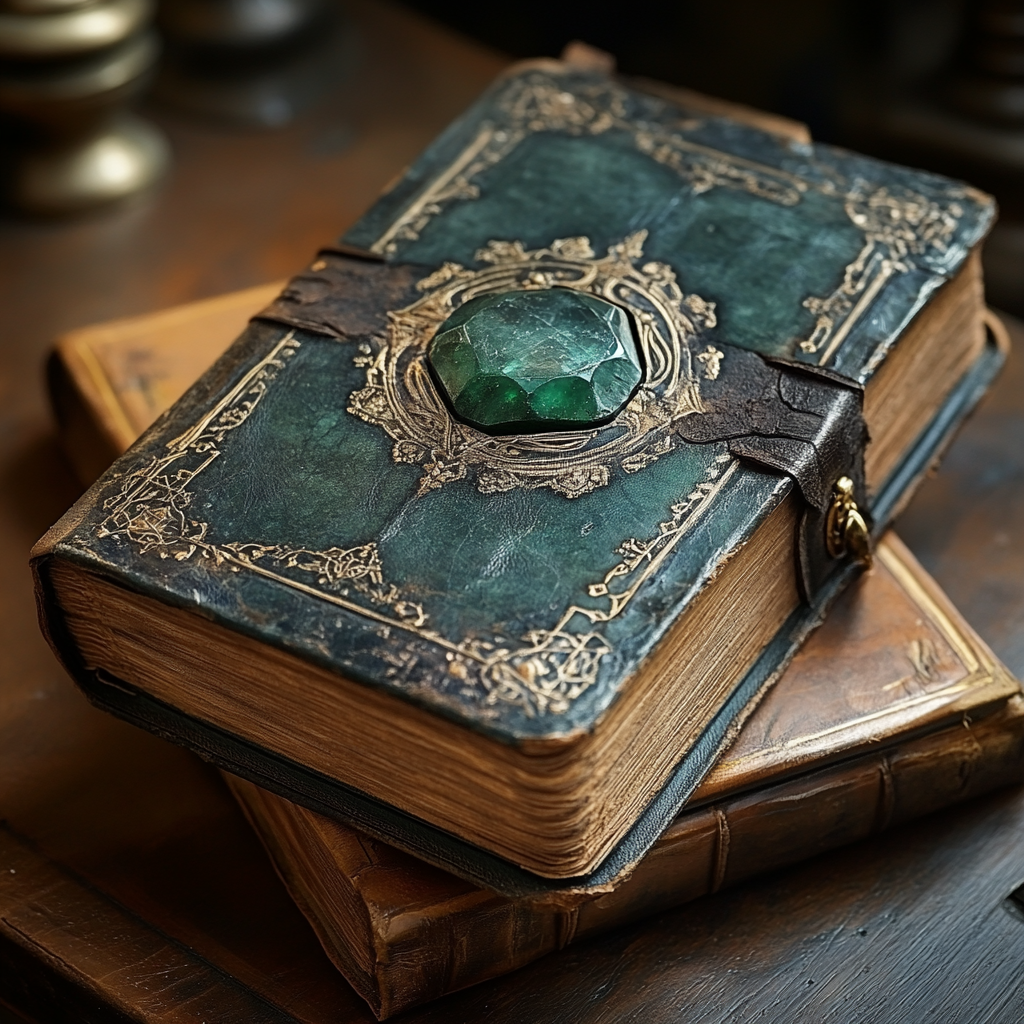
\includegraphics[width=170mm]{logo}\par\end{center}}
\preauthor{\begin{center}\fontsize{14bp}{14bp}\selectfont}
   \postauthor{\par\end{center}}
\predate{\begin{center}}
   \postdate{\par\end{center} }

\title{Addon per Dungeons \& Dragons 5e:\\\textit{Il grimorio del Mago Selvaggio}}
\author{Matteo Scarpa - Fundor333}
\date{\today}


\newcommand{\nomecampagna}{\textit{Kebab e patatine fritte}} %\textit{Alberi del sigillo}}
\newcommand{\mottocampagna}{\textit{Magari anche delle cipolle fritte}}


\begin{document}

\maketitle

\tableofcontents

\mainmatter

\chapter{Introduzione}

\DndDropCapLine{Q}uesto é un piccolo pdf dove vengono inserite tutte le aggiunte che ho creato o raccolto da amici e giocatori per conservarli e averli pronti ad uso. A meno che non sia specificato espressamente, tutto il materiale è stato creato per la 5a edizione di D\&D.

\chapter{Introduzione}

Questo é un piccolo pdf dove vengono inserite tutte le aggiunte che ho creato o raccolto da amici e giocatori per conservarli e averli pronti ad uso.


\chapter{Appendici}
\end{document}
